\documentclass{article} 
\usepackage{listings}
\usepackage{hyperref}
\usepackage{graphicx}
\graphicspath{ {./media/} }
\usepackage{color}
\usepackage[utf8]{inputenc}

\definecolor{codegreen}{rgb}{0,0.6,0}
\definecolor{codegray}{rgb}{0.5,0.5,0.5}
\definecolor{codepurple}{rgb}{0.58,0,0.82}
\definecolor{backcolour}{rgb}{0.95,0.95,0.92}
 
\lstdefinestyle{mystyle}{
    backgroundcolor=\color{backcolour},   
    commentstyle=\color{codegreen},
    keywordstyle=\color{magenta},
    numberstyle=\tiny\color{codegray},
    stringstyle=\color{codepurple},
    basicstyle=\footnotesize,
    breakatwhitespace=false,         
    breaklines=true,                 
    captionpos=b,                    
    keepspaces=true,                 
    numbers=left,                    
    numbersep=5pt,                  
    showspaces=false,                
    showstringspaces=false,
    showtabs=false,                  
    tabsize=2
}
 
\lstset{style=mystyle}

\begin{document} 

\textbf{{Hardware installation Safe-power (all versions of Raspberry
Pi)}}
\vspace{5mm} %5mm vertical space
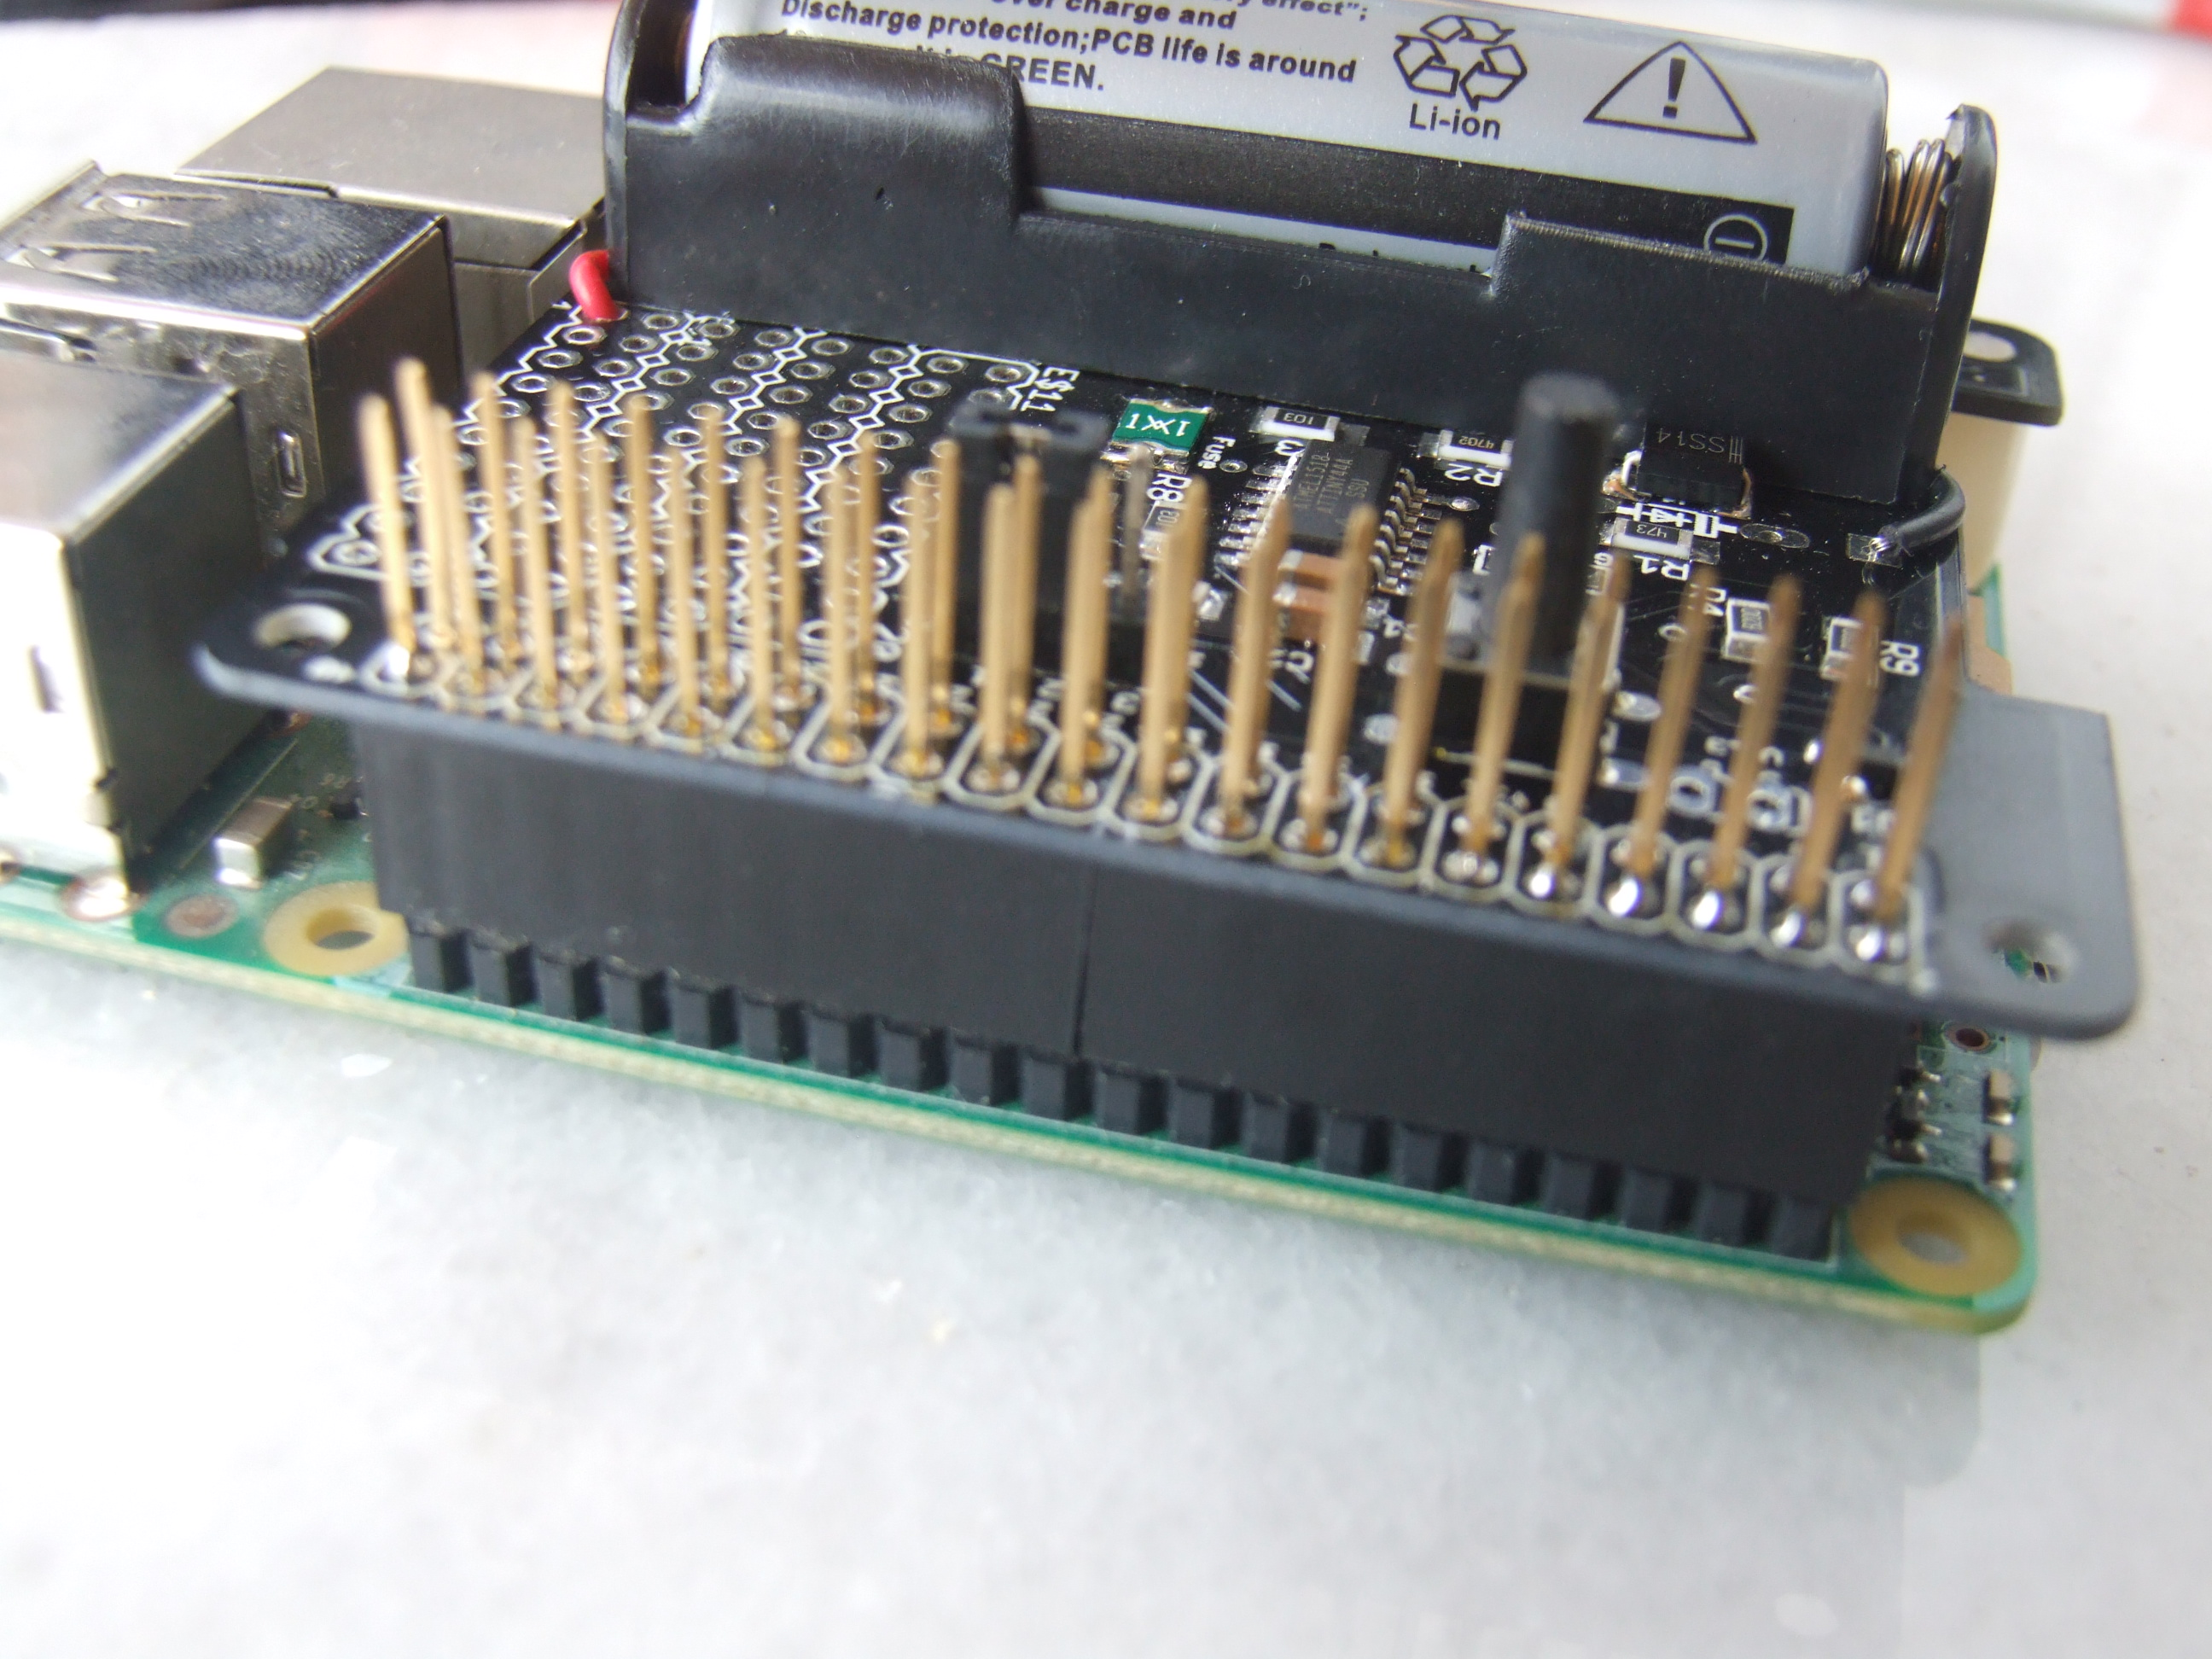
\includegraphics[width=\linewidth]{tg1.jpg}

\begin{enumerate}
\def\labelenumi{\arabic{enumi}.}
\item
  Install the shutdown script as per
  \url{http://safe-power.appspot.com/setup}
\item
  Turn off the Raspberry and disconnect USB power
\item
\vspace{5mm} %5mm vertical space
  insert the AA size LiPo battery, negative pole goes side of the spring




\item
 connect safe-power, Pin1 of Safe-power connects to Pin1 of the
Raspberry
\item
 connect USB power to the Raspberry
\end{enumerate}
Pin 1 Pin1 Raspberry (all models)





\textbf{Operation of Safe-power}


Safe-power monitors constantly the power provided by USB. In case power
fails, there is no delay, and your Raspberry is immediately powered by
the LiPo battery.

On Raspberry version 1 the USB ports and network will cease to work when
on battery power.

If the power cut on USB takes longer than 10 seconds, Safe-power will
send a shutdown signal to the Operating System. This operation will
finish after 30 seconds, the red LED will be on. Battery power will be
cut, and only the microcontroller of Safe-power continues to operate.
This state is indicated by a flash of the red LED every 2 seconds.

When USB power is restored the Raspberry switches back on.

The LiPo battery has it's own charging circuit with 2 LEDs (the small
blue PCB underneath).

Red -- the battery is charging, blue- the battery is full.

\textbf{Warning:} DO NOT replace the provided battery with any other
rechargeable battery, except Lithium Polymer which has a charging
voltage of 4.2V.

\textbf{LED blink codes }




Button for manual shutdown

LED red

LED green

\textbf{Steady green} -- power has been applied, Raspberry boots

\textbf{Blinking green} 2 seconds -- normal operation power ok

\textbf{Blinking red fast} -- power failure detected

\textbf{Steady red} -- shutdown initiated (manual or after power
failure)

\textbf{Blinking red} 2 seconds -- power failure, Raspberry is shutdown

\begin{quote}
\textbf{Blinking red} \textbf{and green} 2 seconds -- system in shutdown
after

manual shutdown by button
\end{quote}

\textbf{Red and green alternating 5 times} -- Safe-power

Microcontroller boots

\textbf{Manual shutdown}

Manual shutdown can be initiated by pressing the button once. The red
LED will turn on for 35 seconds and your Raspberry will shut down the
operating System.

After completed shutdown, red and green will blink. You can now restart
the Operating system by pressing the button.

\textbf{shutdownscript}


%\color{blue}
\begin{lstlisting}[language=Python]
#!/usr/bin/env python
#script to shutdown the raspberry by safe-power raspberry UPS
#add this script to the end of root's crontab in 
#the following way
#  @reboot /path-to/safe-power.py &
# important!! dont forget the "&"  in the end
#in this way the script will be started in the background
# at reboot and safe power will be operational
import RPi.GPIO as GPIO
GPIO.setmode(GPIO.BCM)
import os
import time
# GPIO 11 = pin23 set up as input. 
#It is pulled up to stop false signals
GPIO.setup(11, GPIO.IN, pull_up_down=GPIO.PUD_UP)
# now the program will do nothing until the shutdown
# signal on pin 23
# starts to fall towards zero. This is why we used the pullup
#during this waiting time, your raspberry is not
#wasting resources by polling

try:
    GPIO.wait_for_edge(11, GPIO.FALLING)

#    time.sleep(5)
#    os.system('logger -s " restart after to powerfailure"')
#with the following two lines you could warn all logged users 
#of the shutdown event,
# just adjust the path to your shutdown message
    os.system("wall /etc/shutdownmessage")
#    time.sleep(5)
#    now the system will shut down
    os.system("sudo poweroff")
#except if this script will be cancelled by the user explicitely
except KeyboardInterrupt:
    GPIO.cleanup()       # clean up GPIO on CTRL+C exit
GPIO.cleanup()           # clean up GPIO on normal exit
 
\end{lstlisting}


\end{document}